%%%%%%%%%%%%%%%%%%%%%%%%%%%%%%
% 	   美赛模板,正文部分		 
%          PAPER.tex         
%%%%%%%%%%%%%%%%%%%%%%%%%%%%%%

\documentclass[12pt]{article}

% 请在此填写控制号、题号和标题,年份不需要填(自动以当前电脑时间年份为准)
\usepackage[1923231]{easymcm}\problem{C}   
\usepackage{palatino} % 这个是COMAP官方杂志采用的字体,如不需要可注释掉,以使用默认字体
\usepackage{subfigure}

\title{\large God or evil? A ... model analysing and predicting opioid use}  % 标题
\setlength\parindent{0pt} %default no indent
\newcommand{\upcite}[1]{\textsuperscript{\textsuperscript{\cite{#1}}}}
% 如您参加的是ICM(即选择了D/E/F题),请使用以下的命令修改Summary Sheet题头
% \renewcommand{\contest}{Interdisciplinary Contest in Modeling (ICM) Summary Sheet}

% 正文开始
\begin{document}
%%%%%%%%%%%%%%%%%%%%%%%%%%%%%%%%%%%%%%%%%
%%            请在此填写摘要            %%
%%%%%%%%%%%%%%%%%%%%%%%%%%%%%%%%%%%%%%%%%
\begin{abstract}\small
A non-SPA-style bathtub cannot be reheated by itself, so the water will get noticeably
cooler and users should add hot water from time to time. Based on the existing Partial
Differential Equation (PDE) technique, we construct time-space based temperature model
which can simulate any common condition. And then propose an optimal strategy
for users to keep the temperature even and close to initial temperature and decrease the
water consumption.

Firstly, we construct the PDE-solving model to simulate the temperature distribution
in the bathtub by analyzing the heat loss and confirming the corresponding parameters.
In this part, we consider two kinds of heat transfer, (water-bathtub heat conduction,
water-air heat convection), and the effect of inflow water on the faucet is shown by the
heat source. So we can confirm the boundary conditions of PDE to carry out the next
step.

Secondly, we do parameter testing by free cooling process to ensure the parameters
are in line with the actual condition. Most of the parameters are applicable, and a few
parameters are fine-tuned to make the model more accurate and practicable.
Thirdly, we confirm the optimal strategy by analyzing and comparing the continuous
and discontinuous flow methods, which vary from the temperature and flux. There are
two feasible methods gained from the analyses, one is continuous 42 $^\circ$C water inflow, the
other is turning on and off the faucet with 42 $^\circ$C inflow for 10 minutes.In addition, we
give two more kinds of methods.

At last, we use our model to determine the extent to which our strategy depends on
the factors of the bathtub, the factors of the user, and a bubble bath additive. And we test
the methods by changing the initial temperature. From those results, we further suggest
the users move less and use more bubble bath additive, and turning on the faucet at the
beginning is also a good choice.
\end{abstract}



%%%%%%%%%%%%%%%%%%%%%%%%%%%%%%%%%%%%%%%%%%
% 如不理解以下部分中各命令的含义,请勿修改! %
%%%%%%%%%%%%%%%%%%%%%%%%%%%%%%%%%%%%%%%%%%

%---------以下生成sheet页----------
% 下面的语句可调整全文行距为标准值的0.6倍,请自行使用
%\renewcommand{\baselinestretch}{0.6}\normalsize
\maketitle  % 生成sheet页
\thispagestyle{empty}   % 不要页眉页脚和页码
\setcounter{page}{-100} % 此命令仅是为了避免页码重复报错,不要在意

%---------以下生成目录----------
\newpage
\tableofcontents
\thispagestyle{empty}   % 不要页眉页脚和页码
\newpage

%---------以下生成正文----------
\setlength\parskip{0.8\baselineskip}  % 调整段间距
\setcounter{page}{1}    % 从正文开始计页码
\pagestyle{fancy}		% 摘要请到ABSTRACT.tex中填写

\section*{Memo}
\newpage

\section{Introduction}
\subsection{Problem Background}
Opioids, no matter synthetic ones or non-synthetic ones, play an significant role in our daily life. The proper utilization of opioids helps thousands of people get relieved from their pains. However, misuse of them can really destroy the society. Therefore, it is essential and urgent to gain a better understanding of opioids' spread and influencing factors.

Recent years have witnessed the tremendous growth of opioids cases. How this trend will develop remains an national concern. With data of annual drug use and socio-economic factors in five U.S. states over the past few years, we perform data mining and construct a model to figure out the pattern of opioids use and what contributes to it.

% \subsection{Literature Review}
% A literatrue\upcite{1} say something about this problem ...

\subsection{Our work}
We do such things ...

\begin{enumerate}[\bfseries 1.]
    \item We do ...
    \item We do ...
    \item We do ...
\end{enumerate}

\section{Assumptions and Nomenclature}
\subsection{Assumptions}
Given the lack of data and limitation of our knowledge, we made the following assumption:
\begin{itemize}
    \item We assume that the data after processing is robust for futher use.
\end{itemize}

\subsection{Notations}
The primary notations used in this paper are listed in \textbf{Table \ref{tb:notation}}.
\begin{table}[!htbp]
\begin{center}
\caption{Notations}
\begin{tabular}{cl}
	\toprule
	\multicolumn{1}{m{3cm}}{\centering Symbol}
	&\multicolumn{1}{m{8cm}}{\centering Definition}\\
	\midrule
	$A$&the first one\\
	$b$&the second one\\
	$\alpha$ &the last one\\
	\bottomrule
\end{tabular}\label{tb:notation}
\end{center}
\end{table}

\section{Data Processing}
We are provided with two types of data, the number of drug reports in categories and socio-economic factors. Both of them are specific to counties. The original data contains a lot of redundant and invalid items, which can seriously affect the accuracy and versatility of our model. Thereby, we first apply some data processing techniques before we construct the model.
\subsection{Missing Data Processing}
% In US, each county is assigned a unique five-digit code called FIPS county code. 
In the worksheet about socio-economic factors, there are many cells that contain no valid information at all. We delete columns and rows which contains a lot of useless cells. For other columns and rows, when invalid items appear, we replace it with the average value of the entire sequence.

\subsection{Clustering Counties of Five States}
Since we have detailed number of drug reports, it is not hard to fit a curve to observe the trend of opioid use for each state and for each county. However, we consider this method inappropriate. On the one hand, the sample for only one county is normally fluctuating irregularly, i.e. drug reports of heroin in ACCOMACK, VA was 2, 38, 6 during 2012-2014. It is unnecessary and meaningless to bulid a model when facing such fluctuation. On the other hand, given the large number of all kinds of opioids, even one type change significantly, it is not obvious when viewed as the level of the whole state.

% \begin{figure}[htbp]
% \centering        %居中
% \subfigure[name of the subfigure]{ %第一张子图
% 	\begin{minipage}{7cm}\centering   %子图居中
% 		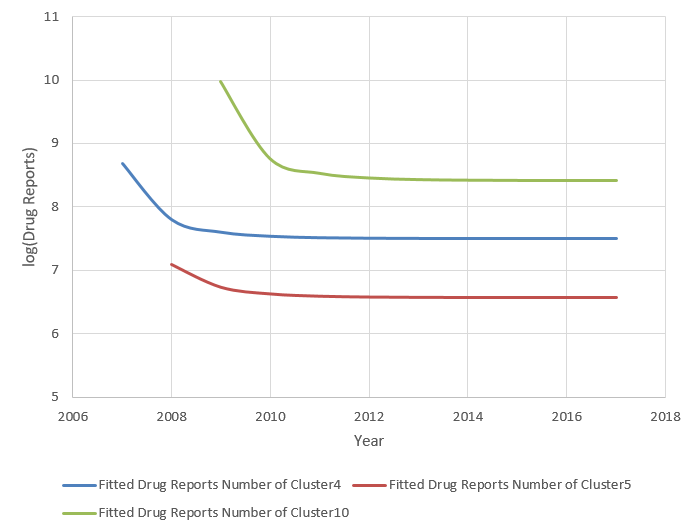
\includegraphics[scale=0.5]{./figures/1.png}  %以pic.jpg的0.5倍大小输出
% 	\end{minipage}}
% \subfigure[name of the subfigure]{ %第二张子图
% 	\begin{minipage}{7cm}\centering %子图居中
% 		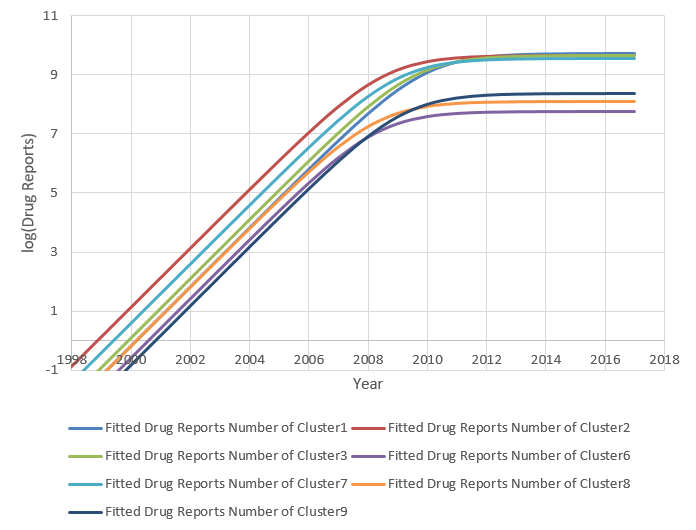
\includegraphics[scale=0.3]{./figures/2.png}  %以pic.jpg的0.5倍大小输出
% 	\end{minipage}}
% \caption{name of the figure} %%大图名称
% \label{fig:1} %图片引用标记
% \end{figure}

Considering that state and county are not suitable for our research, a unit in between is introduced. We put counties on a two-dimensional plane and regard them as nodes. Then, k-means clustering method\upcite{1}, which aims to partion nodes into k clusters minimizing the within-cluster sum of squares, was performed. In our case, we take $k = 10$. The distance of two counties can be computed with their latitude and longtitude retrieved from U.S. Census Bureau\upcite{2}. %TODO: Add cluster figure

\subsection{Combine Indexes of a Socio-economic Factor}
For every year from 2010 to 2016, there are a list of indexes about one single socio-economic factor. For instance, factor ANCERSTRY includes estimate, estimate margin of error, percent, etc. Those indexes all reflect some information of the target factor in some aspects, hence how to rank their importance matters. 

In information theory, entropy represents the information a sequence contains\upcite{3}. So Entropy Weight Method (EWM), which gives each index a weight according to their entropy, is chosen to measure the significance of each index. Before that, we normalize the data given using the following equation.
\begin{equation}
	y_{i} = \frac{x_{i}-min(x_{i})}{max(x_{i}) - min(x_{i})}
\end{equation}
where $x_{i}$ and $y_{i}$ denotes the original sequence and processed sequence.

We apply EWM in the way addressed as follows (Using ANCERSTRY as an example):
\begin{itemize}
	\item Define Estimate, Estimate margin of error, Percent, Percent margin of error of ANCERSTRY is defined as $y_{j}$ ($y_{1}$ means Estimate...). Compute entropy for $y_{j}$: $ E_{j} = -\frac{\sum p_{i}lnp_{i}}{ln(n)}$, where $p_{i}=\frac{y_{ji}}{\sum_{i} y_{ji}}$, $E_{j}$ represents the entropy for each index.
	\item Compute weight for Estimate, Estimate margin of error, Percent, Percent margin of error of ANCERSTRY: $ W_{j} = \frac{E_{j}}{\sum E_{j}}$, where $W_{j}$ represents the weight for each index.
	\item Combine indexes using the weight: $y'_{i} = \sum_{j} W_{j} * y_{ji}$
\end{itemize}
So far, we have combined several indexes of a factor into one $y'_{i}$, and the same can be done to other factors. The newly generated sequence will be reserved for further analysis.

\section{The Models}
\subsection{Model 1}
\subsubsection{Detail 1 about Model 1}
\begin{equation}
    e^{i\theta}=\cos\theta+i\sin\theta.
\end{equation}

\section{Strengths and Weaknesses}
\subsection{Strengths}
\begin{itemize}
    \item Our model takes the idea of clustering, which overcomes the difficulty of analysing either the whole state or one single county.
    \item We take several measures to process the dataset and make it convenient for use, while the authenticity and integrity of data is still maintained.
\end{itemize}

\subsection{Weaknesses}
\begin{itemize}
    \item Nothing yet
 \end{itemize}

\begin{thebibliography}{99}
\addcontentsline{toc}{section}{References}  %引用部分标题("Refenrence")的重命名
\bibitem{1}MacQueen, J. (1967, June). Some methods for classification and analysis of multivariate observations. In Proceedings of the fifth Berkeley symposium on mathematical statistics and probability (Vol. 1, No. 14, pp. 281-297).
\bibitem{2}Gazetteer Files - Geography - U.S. Census Bureau. \texttt{\\https://www.census.gov/geo/maps-data/data/gazetteer.html}
\bibitem{3}Shannon, C. E. (1948). A mathematical theory of communication. Bell system technical journal, 27(3), 379-423.
\bibitem{4}DrugBank. \texttt{https://www.drugbank.ca/drug}
\end{thebibliography}


% ==============以下为附录内容,如您的论文中不需要程序附录请自行删除====================
\clearpage
\begin{subappendices}						% 附录环境
\section*{Apendix: The Source Codes}		% 附录标题可以自行修改
\addcontentsline{toc}{section}{Appendix}  	% 将附录内容加入到目录中

This python program implements k-means clustering.
\lstinputlisting[language={python}, caption=\texttt{k-means.py}]{../code/k-means.py}
% \inputpython{../code/k-means.py}{0}{68}

This MATLAB program is used to calculate the value of variable $a$.
\begin{lstlisting}[language={Matlab}, caption=\texttt{temp.m}]
a = 0;
for i = 1:5
	a = a + 1;
end
\end{lstlisting}

This LINGO program is used to search the optimize solution of 0-1 problem.
\begin{lstlisting}[language=Lingo, caption=\texttt{temp.lg4}]
model:
sets:
WP/1..12/: M, W, X;
endsets
data:
M = 2 5 18 3 2 5 10 4 11 7 14 6;
W = 5 10 13 4 3 11 13 10 8 16 7 4;
enddata
max = @sum(WP:W*X);
@sum(WP: M * X)<=46;
@for(WP: @bin(X));
end
\end{lstlisting}

\textbf{\textcolor[rgb]{0.98,0.00,0.00}{Input matlab source:}}
% \lstinputlisting[language=Matlab]{../code/matlab-test.m}

\end{subappendices}
% =================================================================================



\end{document}